\documentclass{beamer}
 
\usepackage[utf8]{inputenc}
\usepackage{hyperref}
\usetheme{Madrid}
\usecolortheme{beaver}

\title{More on Graphs}
\subtitle{Minimum Spanning Tree and Dijkstra's Algorithm}
\author[Carocari, Fabris, Lotito]
{Giulia Carocari, Giacomo Fabris, Francesco Lotito}
\institute[UniTN]{Università degli Studi di Trento}
\date[March 27, 2019]
{ICPC Training @ UniTN\\ Day 3 - March 27, 2019}
 
 
 
\begin{document}
 
  \frame{\titlepage}
  \begin{frame} 
      \frametitle{Table of Contents}
      \tableofcontents
  \end{frame}
  \AtBeginSection[]
  {
    \begin{frame}
      \frametitle{Table of Contents}
      \tableofcontents[currentsection]
    \end{frame}
  }

  \section{Solutions from last week's contest}
  \begin{frame}
  \frametitle{A - Counting Stars}
  \begin{block}{Problem definition}

  \begin{itemize}
    \item The sky is a grid of  $N\cdot M$ cells, each containing a piece of sky ('\#') or star ('-').
    \item A star is a section of the sky made of one or more adjacent (up/down or left/right) starry pixels.\\
    \item How many stars are there in this portion of sky?
  \end{itemize}
  \end{block}
  \pause
  \setbeamercolor{block title}{use=structure,fg=white,bg=cyan!75!black}
  \begin{block}{Solution}
    Count connected components on a graph where adjacent star cells in the grid are neighbouring nodes.
  \end{block}
  \alert{Remarkable applications of such visits on graphs:}
  You may want to consider \href{http://disi.unitn.it/~montreso/asd/compiti/18-01-31.compito.pdf}{ASD 2018/01/31} (exercise 3).
  \end{frame}

  \begin{frame}
    \frametitle{B - Dominos}
    \begin{block}{Problem definition}

    \begin{itemize}
      \item Consider a field covered in domino tiles
      \item We are given precedence rules on what piece makes what other peace fall.
      \item What is the minimum number of times we have to knock over a piece in order to make them all fall?
    \end{itemize}
    \end{block}
    \pause
    \setbeamercolor{block title}{use=structure,fg=white,bg=cyan!75!black}
    \begin{block}{Solution}
      Find strongly connected components (Kosaraju or Tarjan) and count those that do not have any entering
      edge from other SCC.
    \end{block}
  \end{frame}

  \begin{frame}
    \frametitle{C - Erdos Numbers}
    \begin{block}{Problem definition}
      Find the Erdos number of the listed authors, given their set of co-authors.\\
      The Erdos number of a person is the minimum length of a co-authoring chain that connects him/her to Paul Erdos.
    \end{block}
    \pause
    \setbeamercolor{block title}{use=structure,fg=white,bg=cyan!75!black}
    \begin{block}{Solution}
      Run a BFS on the input graph, assigning to each author his distance from the starting node (PAUL\_ERDOS).
    \end{block}
    \alert{Programming tips:} Implement the graph as a hash map (\texttt{unordered\_map} in \texttt{C++}), where the ID of a node is the author's name.
    The name of each node in the graph is hashed to a vector of adjacent people.
  \end{frame}

  \begin{frame}
    \frametitle{D - Arctic Network}
    \begin{LARGE}
      \begin{center}
        We will speak about this problem and its solution in a few slides.
      \end{center}
    \end{LARGE}
  \end{frame}

  \begin{frame}
    \frametitle{E - Family DAG}
    \begin{LARGE}
      \begin{center}
        As no one solved it, we will leave you one more week to work on it.
      \end{center}
    \end{LARGE}
  \end{frame}

  \begin{frame}
    \frametitle{F - Getting Gold}
    \begin{block}{Problem definition}
      Given the map of a dungeon, featuring walls (\#), floor tiles (.), gold (G) and traps (T), find the maximum amount of gold a person can collect
      without ever risking to fall into a trap.\\
      \alert{NOTE:} The player can detect traps if they are in an adjacent cell, but he will not know in what cells they are located.
    \end{block}
    \pause
    \setbeamercolor{block title}{use=structure,fg=white,bg=cyan!75!black}
    \begin{block}{Solution}
      If the player detects a trap, the only safe move he can perform is to go back to where he came from.
      To find all places safely reachable, start a flood fill from the initial position (P), ending the visit whenever the player hits a wall or detects a trap.
      Keep a gold counter to track the loot you collected.
    \end{block}
  \end{frame}
  
  \section{Minimum Spanning Tree}
  \begin{frame}
  \frametitle{Minimum Spanning Tree}
    \begin{block}{Problem definition}
      Given a graph $G=(V,E)$, with a weight function $w:E\rightarrow \mathbb{R} ^+$, 
      find a subset $E'$ of $E$ such that $(V,E')$ is a \textbf{tree} and
      $$W=\sum_{e'\in E'} w(e')$$ is minimal.
    \end{block}
    \pause
    \alert{Greedy choice theorem.} \begin{itemize}
      \item{Base case:} Every 1-vertex graph is a minimum spanning tree.
      \item{Inductive step:} Given a MST $(V',E')\subset (V,E)$, we can connect $v \in V\setminus V'$ by adding 
        to $E'$ the edge $e=(v,v')$ such that $w(e)$ is minimal with respect to all edges connecting $v$ to a node in $E'$. 
    \end{itemize}
  \end{frame}

  \begin{frame}{Two greedy approaches}
    \begin{block}{Kruskal's Algorithm}
      Keep all edges in a \texttt{MinPriorityQueue} to add them in incresing order to the minimum spanning tree.\\
      Use Merge-Find Sets to detect cycles when adding edges to the MST: when adding an edge to the MST perform a merge of the two sets containing the endpoints of the edge itself.
      (if the two endpoints of the edge are in the same set, we will get a cycle).
    \end{block}
    \begin{block}{Prim's Algorithm}
      Start from a random root of the minimum spaning tree and add the minimum weight edge that departs from the current MST.  
    \end{block}
  \end{frame}

  \begin{frame}{Prim's Algorithm}
    \begin{itemize}
      \item Select a root, add all its edges in a \texttt{PriorityQueue} sorted by increasing weight
      \item Pop from the queue, add edge to the MST if it connects a vertex which has not been connected yet
    \end{itemize}
    \begin{figure}[!htb]
      \center{
        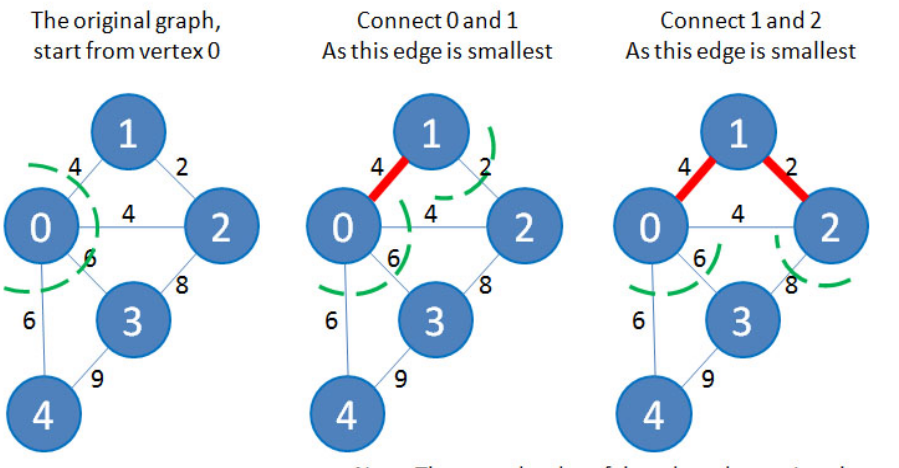
\includegraphics[width=70mm]{prim1}
        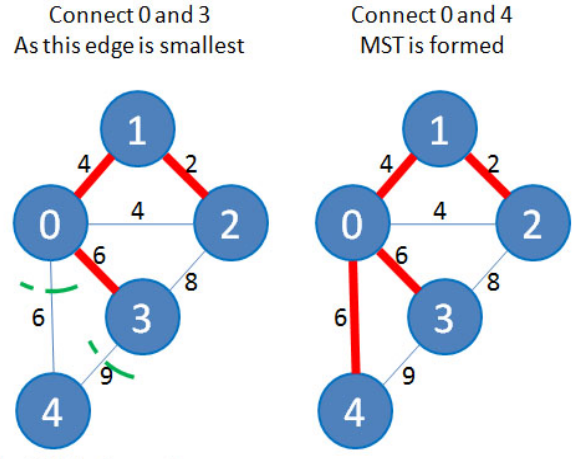
\includegraphics[width=45mm]{prim2}
      }
    \end{figure}
  \end{frame}

  \begin{frame}{Arctic Network}
    \begin{block}{Problem definition}
      Given a set of $N$ outposts in the Arctic and a number of $S$ available satellite channels,
      we want to compute the maximum power $D$ (aka distance range) required by the radio transceivers that have to connect every outpost, directly or indirectly.
      \alert{NOTE:} if an outpost is equipped with a satellite channel it does not need a transceiver.
    \end{block}
    \pause
    \setbeamercolor{block title}{use=structure,fg=white,bg=cyan!75!black}
    \begin{block}{Solution}
      Run Prim/Kruskal on the complete graph of the outposts (weight is given by the distance of every pair of nodes). 
      After you have obtained the MST, sort its edges by increasing weight and return the edge with index $N-S-2$.
    \end{block}
  \end{frame}
  
  \section{Single Source Shortest Path}
  \begin{frame}
  \frametitle{Dijkstra's Algorithm}
    \begin{block}{Problem definition}
      Given a graph $G=(V,E)$, with a weight function $w:E\rightarrow \mathbb{R} ^+$, 
      find the length of the shortest path from a source $s$ to all other nodes in $V$.
    \end{block}

    \alert{NOTE:} Dijkstra's Algorithm works well only with positive weights on edges, for some reasons that
    you will see in class. Other algorithms (e.g. Bellman-Ford) have slight less strict constraints (the graph cannot contain negative-weight cycles),
    but we shall discuss them another time.
  \end{frame}

  \begin{frame}
    \frametitle{Dijkstra's Algorithm}
      \begin{huge}
        \begin{center}
          Enough talking... Let's get to the code!
        \end{center}
      \end{huge}
    \end{frame}

\end{document}